%% IMPORTANT! COMPILE WITH -shell-escape option for ffcode to work

\documentclass[a4paper,11pt]{article}
% Useful packages
\usepackage{amsmath}
\usepackage{amssymb}
\usepackage[utf8]{inputenc}
\usepackage[pdftex]{graphicx}
\usepackage{etoolbox}
\usepackage[svgnames]{xcolor}
\usepackage{tcolorbox}
\usepackage{fancyhdr}
\usepackage{matlab-prettifier}
\usepackage{enumerate}
\usepackage[shortlabels]{enumitem}
\usepackage{amsthm}
\usepackage{ffcode}

% Page size
\textwidth=170mm
\oddsidemargin=0mm
\evensidemargin=\oddsidemargin
\textheight=230mm
\topmargin=-10mm
%Section numbering
\setcounter{secnumdepth}{-1}
%opening
\title{EITF75: Lab 2A&B Report}
\author{Ola Davidsson and Emil Lantz}
\begin{document}
\raggedright
\maketitle
\section{Preparation exercises}
\subsection{Problem 1}
\subsubsubsection{a}
\[
x(n) = [1, 1, -1, 1, 1, -1, 1, -1, -1]
\]
\subsubsection{b}
\[
Data Rate (R_d) = \frac{Data bits}{sample}\cdot\frac{sample}{second} = 10^{6}
\]
\[
F_s = \frac{R_d}{1} = 10^6
\]
\subsubsection{c}
\[
samples = \frac{samples}{s}\cdot s = 10^6\cdot\frac{300}{3\cdot10^8} = 1 sample
\]
\subsubsection{d}
\[
r(n) = s(n) + \alpha\cdot s(n-1)
\]
\subsubsection{e}
\[
h(n) = \delta (n) + \alpha\delta(n-1)
\]
\subsubsection{f}
Depends on the $\alpha$ value. For values below 1 it is possible. For very big values we can also just see it the bit after. 
\subsection{Problem 2}
\subsubsection{a}
\[
H_r(z) = \frac{1}{H(z)}
\]
\subsubsection{b}
\[
H_t(z) = \frac{1}{H(z)} 
\]
\subsubsection{c}
Should be better on the transmitter because if we let the noise affect the filtered signal there´s a greater chance that the noise is enough to either move a 1 to a -1 or a -1 to a 1. 
\subsection{Problem 3}
\subsubsection{a}
\[
\Tilde{s}(n) = [\underline{1}, 2, 3, 4]
\]
\[
s(n) = [\underline{3}, 4, 1, 2, 3, 4]
\]
\subsubsection{b}
\[
r(n) = s(n)*h(n)
\]
With table method we get
\[
r(n) = [3, 4, 4, 6, 4, 6, 3, 4]
\]
\subsubsection{c}
\[
r_c(n) = \tilde{s}(n) \circledast h(n)
\]
With table method we get.
\[
r_c(n) = [4, 6, 4, 6]
\]
\subsubsection{d}
If we removing the first and last L-1 numbers in r(n) we can see that 
\[
r_c(n) = r(n)
\]
\subsection{Problem 4}
\subsubsection{a}
\subsubsubsection{1}
We force x(n) into frequency plane and creating 
\[
x(k) = \tilde{S}(k)
\]
\subsubsubsection{2}
\[
x_{IDFT}(n) = \frac{1}{N} \sum_{k=0}^{N-1} X(k) \cdot e^{\frac{j2\pi k n}{N}} = \tilde{s}(n)
\]
\subsubsubsection{3}
We then add the cp to create s(n)
\subsubsection{b}
\[
\tilde{R}(k) = \tilde{S}(k) \cdot H(k)
\]
\subsubsection{c}
\[
H(0), H(1), H(N-1)
\]
\subsubsection{d}
\[
\frac{1}{H(n)}
\]
\section{Lab 1A}
\subsection{Lab task 1}
To plot and check the 'statistics' of the generated bit sequence, the following MATLAB code was used
\begin{ffcode}
%% task 1
clc; clear
nbr_of_bits = 64;
data = rand(1,nbr_of_bits);
data = zeroOne(data);
stats = sum(data)
figure(1)
stem(data(1:64))
\end{ffcode}
Where zeroOne is a predefined function (found in appendix)

For small values of 'nbr\_of\_bits', 'stats' varied quite alot. However, for very large values (i.e. 50000), 'stats' could be seen tending towards zero.


Plots of the input signal and transmit bits can be seen in figure 1 and 2 respectively. These were plotted using MATLABs CLI since zeroOne converts the signal to transmit form instantly.

\begin{figure}[H]
    \hspace{-40pt}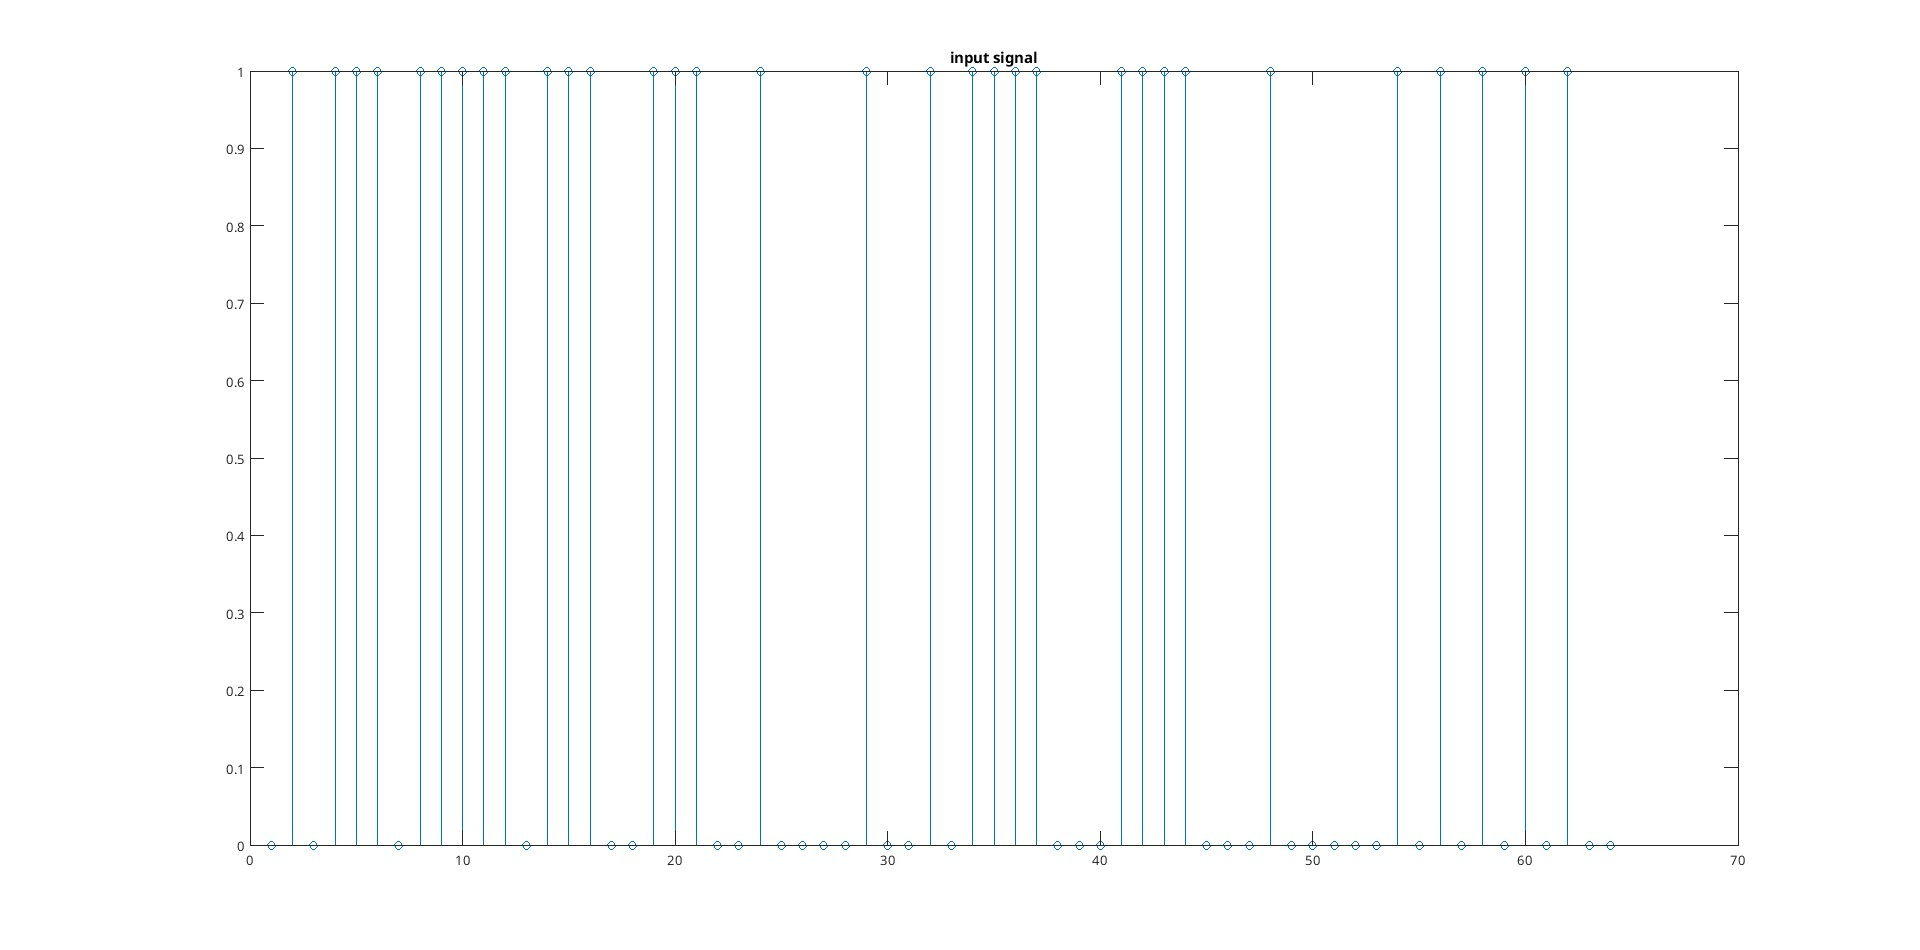
\includegraphics[scale=0.28]{./images/inputsignal.jpg}
    \caption{Stem-plot of input signal used in lab 2A}
    \label{fig:my_label}
\end{figure}

\begin{figure}[H]
    \hspace{-40pt}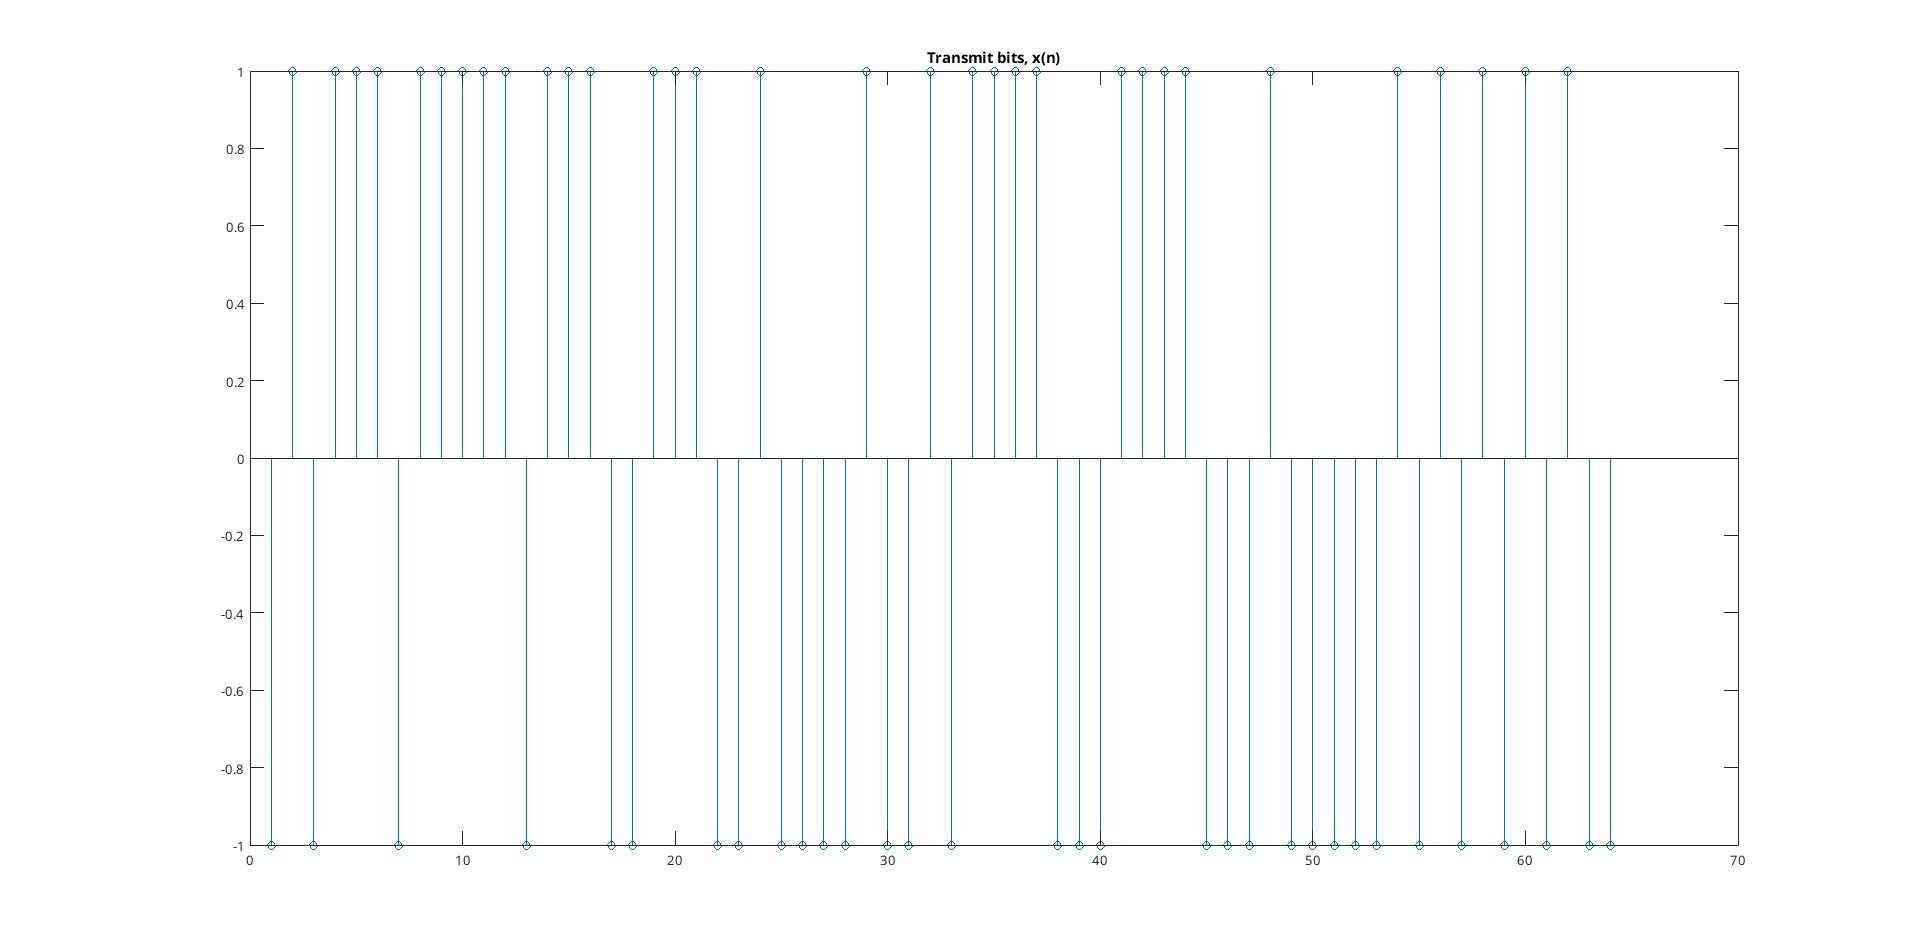
\includegraphics[scale=0.28]{./images/transmitbits.jpg}
    \caption{Stem-plot of transmit bits x(n), used in lab 2A}
    \label{fig:my_label}
\end{figure}

Looking at figure 1 & 2, one can see that the plots match up with the algorithm given in the task. All points where input is 0 has been converted to -1.

\subsection{Lab task 2}
Calculating and plotting the receiver signal (for all three values of $\alpha$) was achieved through
\begin{ffcode}
%% Task 2
alpha = [0, 0.5, 0.99];
figure(3)
subplot(4, 1, 1)
stem(data)
title('transmit bits x(n)')

for i = 1:length(alpha)
recv = trim_end(conv(data, [1 alpha(i)]));
subplot(4, 1, i+1)
stem(recv)
title(sprintf('Reciever signal (α = %.2f)', alpha(i)))
end
\end{ffcode}


The plot yielded can be seen in figure 3
\begin{figure}[H]
    \hspace{-50pt}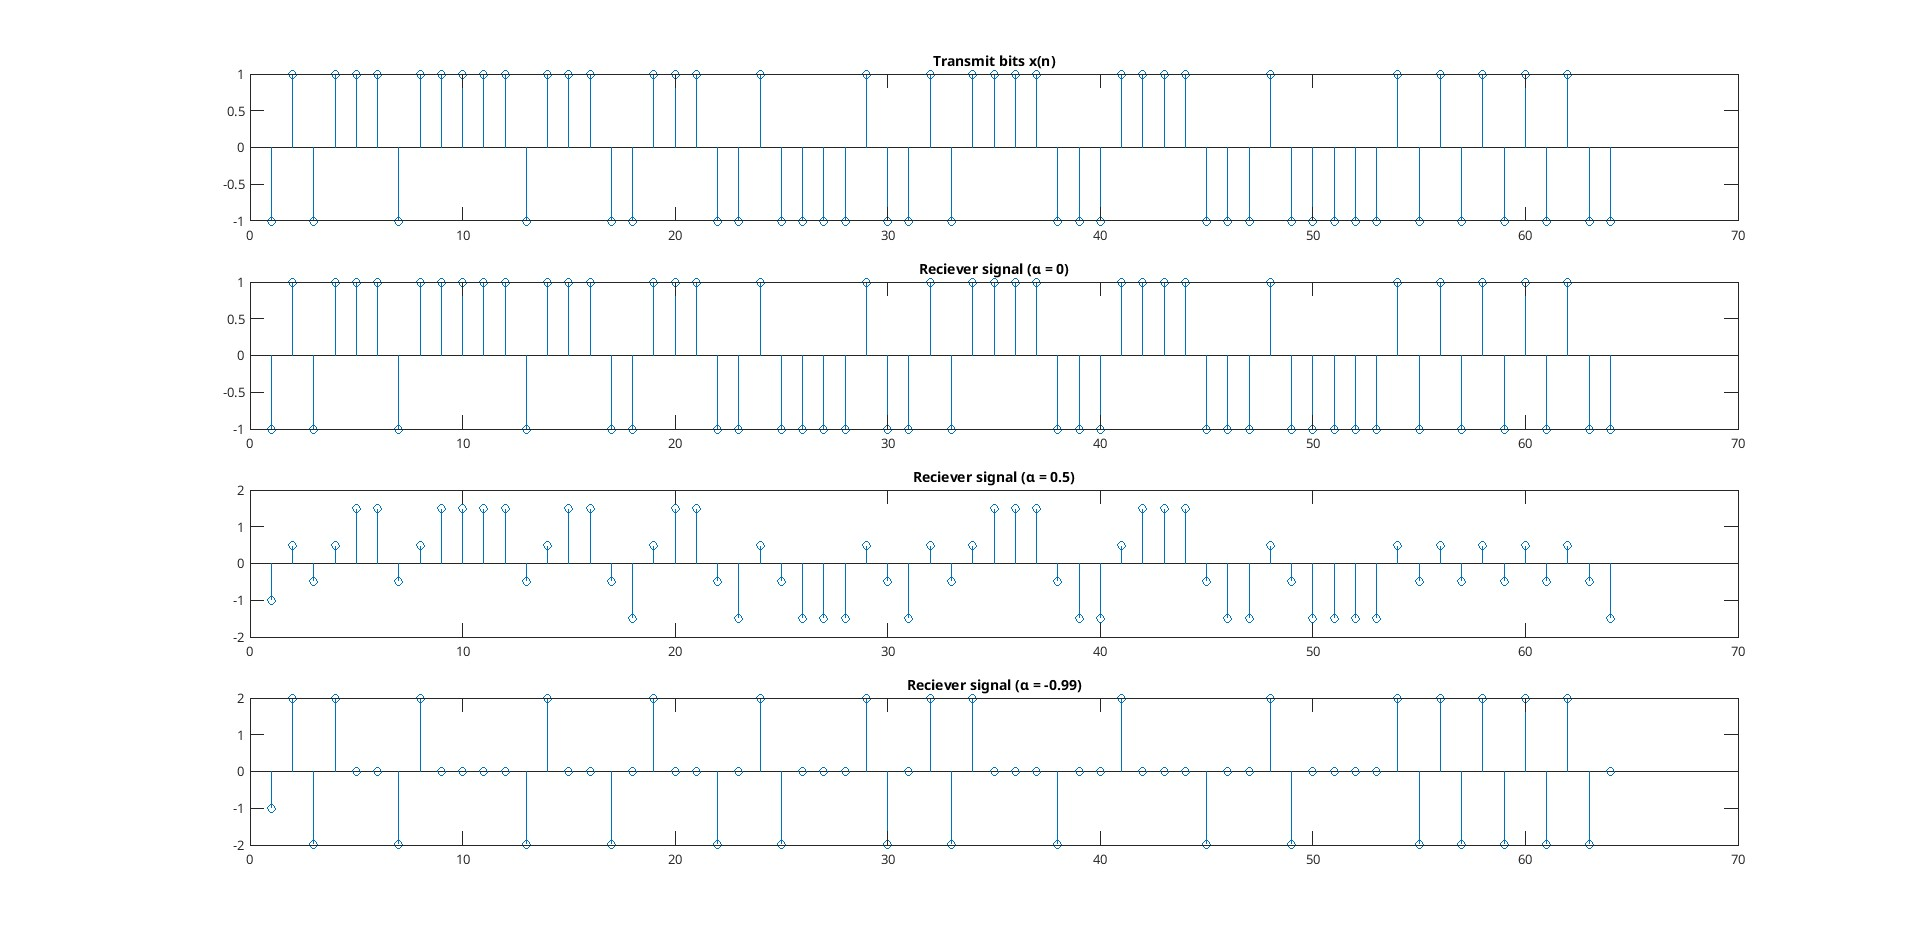
\includegraphics[scale=0.28]{./images/task2_subplots.jpg}
    \caption{Subplots of stem-plots given in task 2}
    \label{fig:my_label}
\end{figure}

Looking at these plots, one can see where the two signals ($\delta(n)$ and $\alpha\delta(n-1)$) add together, giving an amplitude of $A = 1+\alpha$. Looking at this, $\alpha$ can easily be figured out by looking at the plots.


\subsection{Lab task 3}
The MATLAB code used for implementing our detection algorithm can be seen below
\begin{ffcode}
%% Task 3

for i=1:length(alpha)
    H_z = [1, alpha(i)];
    H_t = filter(1, H_z, data);
    y_t = trim_end(conv(H_z, H_t));
    receiver_hr = trim_end(conv(data, H_z));
    y_r = filter(1, H_z, receiver_hr);

    %plot transmitter
    subplot(3, 2, 2*i - 1)
    stem(y_t)
    title(sprintf('transmitter signal, (α = %.2f)', alpha(i)))
    
    %plot receiver
    subplot(3, 2, 2*i)
    stem(y_r)
    title(sprintf('receiver signal, (α = %.2f)', alpha(i)))

    %add noise
    y_t_noisy = noise(y_t, 0.25);
    y_r_noisy = filter(1, H_z, noise(receiver_hr, 0.25));

    diff_yt = bits_diff(restructure(y_t_noisy), data);
    fprintf("Diff between restructured y(t) and x(n) (α = %.2f): %.3f \n", ...
        alpha(i), diff_yt)

    diff_yr = bits_diff(restructure(y_r_noisy), data);
    fprintf("Diff between restructured y(r) and x(n) (α = %.2f): %.3f \n\n", ...
        alpha(i), diff_yr)
end
\end{ffcode}

The algorithm worked almost flawlessly for clean signals, and presented some error when noise was added to the signal.

Looking at data generated from running the code, one can see that implementing noise reduction on the transmitter end of the system yields a more accurate representation (than the receiver end) of the original transmit bits, x(n). 

\subsection{Lab task 4}
MATLAB code for generating the signals shown in figure 3 (of the lab instructions) was as follows 
\begin{ffcode}
%% Task 4
clc; clear; addpath('./functions/')
N = 64;
L = 2;
x_n = rand(1, N);
x_n = zeroOne(x_n);
alpha = [0 0.5 -0.99];
%inverse DFT
sf_n = ifft(x_n, N);
%CP
cp = sf_n(end - (L-2):end);
s_n = [cp, sf_n];

for i=1:length(alpha)
    H_z = [1, alpha(i)];

    r_n = conv(s_n, H_z);
    rf_n = r_n(L:end-(L-1));
    y_n = fft(rf_n, N);
    h_n = [1, alpha(i), zeros(1, 62)];

    H_k = fft(h_n, N);
    xn_fig4 = y_n ./ H_k;
    error = bits_diff(sign(real(xn_fig4)), x_n);

    fprintf("Difference between Re(x(n)) using model " + ...
        "from figure 3, and x(n) (α = %.2f): %.3f \n\n", alpha(i), error);
end
\end{ffcode}

On line 74 to line 76, the algorithm from fig 4 of the instructions is implemented. Running the code will print the error of the algorithm, showing minimal errors, meaning that the OFDM system worked quite well, as expected.
\subsection{Lab Task 5}
Task 5 was completed using the following MATLAB code
\begin{ffcode}
%% Task 5
for i=1:length(alpha)
    H_z = [1, alpha(i)];

    r_n = conv(s_n, H_z);
    rn_noise = noise(r_n, 0.25/64);

    rf_n = rn_noise(L:end-(L-1));
    y_n = fft(rf_n, N);
    
    h_n = [1, alpha(i), zeros(1, N-2)];
    H_k = fft(h_n, N);

    xn_noise = y_n ./ H_k;

    error = bits_diff(sign(real(xn_noise)), x_n);
    
    fprintf("Difference between Re(x(n)) using model " + ...
         "from figure 4, and x(n) (α = %.2f): %.3f \n\n", alpha(i), error);

end
\end{ffcode}

Bit comparison (printed using the code from lab task 4) of the recovered signal with the original signal can be seen in figure 4. The same comparison, with added noise can be seen in figure 5.

\begin{figure}[H]
    \includegraphics[scale=0.9]{./images/task_5.png}
    \caption{Bitwise error for noise-free ODFM detection algorithm}
    \label{fig:my_label}
\end{figure}

\begin{figure}[H]
    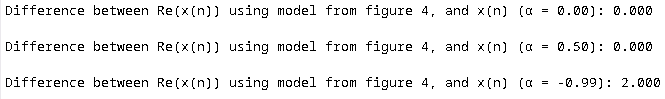
\includegraphics[scale=0.9]{./images/task5_noise.png}
    \caption{Bitwise error for noise-free ODFM detection algorithm}
    \label{fig:my_label}
\end{figure}

To compare the algorithms from lab task 2 and lab task 5, the code was run 100 times using for loops, and the errors were added up and compared. The transmitter error from lab task 2 was almost identical to the OFDM error (OFDM was slightly better). OFDM was, however, nearly seven times better than the receiver signal.

\pagebreak
\section{Appendix}
\subsection{MATLAB functions}
\begin{ffcode}
%% Functions
function fixed = zeroOne(Vector)
Vector = Vector < 0.5;
Inverterare = Vector -1;
fixed = Vector + Inverterare;
end

function back = restructure(Vector)
back = Vector > 0;
Inverterare = back -1;
back = back + Inverterare;
end

function diff = diff(Vector1, Vector2)
diff = sum(Vector1~=Vector2);
end

function noised = noise(Vector, sigma_squared)
noised = sqrt(sigma_squared)*randn(1,length(Vector)) + Vector;
end

function trimmed = trim(Vector)
trimmed = Vector(1:end-1);
end
\end{ffcode}
\end{document}